\documentclass[
%draft,
11pt,
titlepage,
reqno,
%	oneside,
%	twocolumn
]{article}%Draft option puts "slugs" in the margin for overfull lines

%\usepackage{newlattice}%custom package by Gratzer. Use with amsart See book for details.
%Packages loaded by amsart:
%\usepackage{amsmath}%This loads amsbsy, amsopn, amstext
%\usepackage{amsfonts}
\usepackage{amsthm}%This loads amsgen
\usepackage{amsxtra}
\usepackage{geometry}

%\usepackage{pdfsync}
%\usepackage{upref}
%\usepackage{amsidx}
%\usepackage{stmaryrd} %This adds small left arrows for accents that more closely mirror the \vec command
\usepackage{amssymb}
\usepackage{mathtools}
\usepackage{latexsym}
\usepackage{amsmath}

\usepackage{exscale}
\usepackage{amscd} %commutative diagrams
\usepackage{dcolumn} %to get decimal places aligned in tables
\usepackage{array}
\usepackage{tabularx}
%\usepackage{MnSymbol} %dashed arrows and more - see documentation
\usepackage[mathscr]{eucal}
\usepackage[english]{babel}
\usepackage[pdftex]{graphicx}
\usepackage{booktabs}%for nice tables (see discuss at https://people.inf.ethz.ch/markusp/teaching/guides/guide-tables.pdf). For details see https://ctan.org/pkg/booktabs.
% A FANCY TABLE
% \begin{table*}\centering
% \ra{1.3}
% \begin{tabular}{@{}rrrrcrrrcrrr@{}}\toprule
% & \multicolumn{3}{c}{$w = 8$} & \phantom{abc}& \multicolumn{3}{c}{$w = 16$} &
% \phantom{abc} & \multicolumn{3}{c}{$w = 32$}\\
% \cmidrule{2-4} \cmidrule{6-8} \cmidrule{10-12}
%     & $t=0$    & $t=1$    & $t=2$  & & $t=0$    & $t=1$    & $t=2$   & & $t=0$    & $t=1$   & $t=2$\\ \midrule
% $dir=1$\\
% $c$ & 0.0790   & 0.1692   & 0.2945 & & 0.3670   & 0.7187   & 3.1815  & & -1.0032  & -1.7104 & -21.7969\\
% $c$ & -0.8651  & 50.0476  & 5.9384 & & -9.0714  & 297.0923 & 46.2143 & & 4.3590   & 34.5809 & 76.9167\\
% $dir=0$\\
% $c$ & 0.0357   & 1.2473   & 0.2119 & & 0.3593   & -0.2755  & 2.1764  & & -1.2998  & -3.8202 & -1.2784\\
% $c$ & -17.9048 & -37.1111 & 8.8591 & & -30.7381 & -9.5952  & -3.0000 & & -11.1631 & -5.7108 & -15.6728\\
% \bottomrule
% \end{tabular}
% \caption{Caption}
% \end{table*}
\usepackage{subcaption}%for tables and such
\usepackage{lipsum} %for preventing breaks and such
%\usepackage{pgf,pgfarrows,pgfnodes,pgfshade}
\usepackage{setspace} %Turn ON for editing
%\usepackage{verbatim}
%\usepackage{enumerate}
%\usepackage{xspace}`
%\usepackage{longtable}
%\usepackage{epstopdf}
%\usepackage[authoryear]{natbib}
%\usepackage{lscape}
\usepackage{natbib}
\bibliographystyle{chicago}

%\theoremstyle{plain}
\newtheorem{acknowledgement}{Acknowledgement}
\newtheorem{assumption}{Assumption}
\newtheorem{axiom}{Axiom}
\newtheorem{case}{Case}
\newtheorem{claim}{Claim}
\newtheorem{conclusion}{Conclusion}
\newtheorem{condition}{Condition}
\newtheorem{conjecture}{Conjecture}
\newtheorem{corollary}{Corollary}
\newtheorem{criterion}{Criterion}
\theoremstyle{definition}
\newtheorem{definition}{Definition}
\newtheorem{econjecture}{Empirical Conjecture}
\newtheorem{example}{Example}
\newtheorem{exercise}{Exercise}
\newtheorem{lemma}{Lemma}
%\theoremstyle{remark}
\newtheorem{remark}{Remark}
\newtheorem*{notation}{Notation}
\newtheorem{proposition}{Proposition}
\newtheorem{theorem}{Theorem}
\newtheorem*{main}{Main Theorem}
\newtheorem{solution}{Solution}
\newtheorem{summary}{Summary}
%\newenvironment{proof}[1][Proof]{\noindent\textbf{#1.} }{\ \rule{0.5em}{0.5em}}

\newcommand{\BigFig}[1]{\parbox{12pt}{\Huge #1}}%See Gratzer l. 2442 (for matrix)
\newcommand{\BigZero}{\BigFig{0}}

\doublespacing %This is a command from the SetSpace package

\geometry{letterpaper}
\setlength{\oddsidemargin}{0in}
\setlength{\topmargin}{0in}
\setlength{\topskip}{0in}
\setlength{\headsep}{0in}
\setlength{\headheight}{0in}
\setlength{\textwidth}{6.5in}
\setlength{\textheight}{8.75in}

%junk comment for Git

\begin{document}
	
\title{Intentional Awareness\thanks{}
}
\author
{
Brian Epstein \\Tufts University, Medford
\and 
Michael D.\ Ryall \\University of Toronto 
}
\date{\today}
\maketitle
	
%\begin{abstract}
	
%\end{abstract}
	
%\doublespacing
\def\baselinestretch{1.5}\small\normalsize
\newcommand{\ra}[1]{\renewcommand{\arraystretch}{#1}}%for tables
\newpage



\section{Introduction}\label{sec: intro}
This note presents the full mathematical description of the intentional awareness model. 
It is not meant to be a paper.
Rather, it is a full elaboration of a model that can be summarized or referred to in a paper.
Some discussion of how certain mathematical objects are intended to be interpreted is provided (though, these descriptions are not at the same level of detail required for a paper).

In what follows, we develop a four-phase model of intentional acts. 
The essential aim of this formalism is to take seriously the cognitive constraints we face as finite, material beings.
In particular, we proceed from the uncontroversial claim that, at any given moment, an individual can only  attend to some finite number of conscious concerns. 
We say that an individual is \textit{aware} of the matters toward which his or her attention is directed.
Under constrained awareness, intentions take on an important role that is distinct from beliefs and desires.

Our approach refines some existing discussions on this topic by distinguishing between states and acts. 
A state is a snapshot of the world at a given moment in time that describes the status of all the features that are relevant to the situation at hand. 
An act is a procedure that unfolds over time. 
Starting in a state of the world at time $t$, the willful acts of individuals and the brute acts of Nature jointly determine the state of the world at time $t+1$.
This interaction is elaborated in the following sections.

Acts include both efforts that are inherently invisible to others (i.e., mental activities such as deliberating, judging, and choosing) and those that are observable (e.g., enrolling in a graduate course).
We refer to the latter as actions to distinguish them from the sorts of acts that can only be observed by the acting individual. 
Thus, actions are a subcategory of act.
All forms of act have the power to influence future  states of the world.

An individual in our model proceeds from an initial state of the world at time $t$ to a future action according to the following sequence of phases. Each phase is assumed to take \textit{at least} one unit of time. During a phase, all individuals and Nature may act, thereby bringing the world to a new state. Individuals recall their experiences from earlier phases in later phases.
\begin{enumerate}
	\item \textbf{Orientation:} Contemplating their awareness, beliefs, knowledge, and preferences as featured in the state at $t$, individuals identify the future states toward which they may attempt to influence events through their actions; we refer to these future states as potential \textit{goals} toward which they may move. In this phase, individuals may choose to organize  available information and to shift the discretionary scope of their awareness in such a way as best to support an act of deliberation---or, they may choose to wait and evolve to a new state in which they may engage in another act of orientation.
	
	The world evolves to a new state.
	\item \textbf{Deliberation:} Contingent upon the act of orientation to engage in an act of deliberation and given the awareness, beliefs, knowledge, and preferences featured in this new state, individuals conduct an analysis to determine which goal should be pursued. Individuals screen out infeasible and dominated goals and then rank-order the remaining ones according to their preferences. The completion of this analysis is a conclusion about which goal to pursue. If no goal is best, revert to a new act of orientation.
	
	The world evolves to a new state.
	
	\item \textbf{Judgment:} Contingent upon the goal selected as best and given the awareness, beliefs, knowledge, and preferences featured in this new state, individuals decide whether to pursue the goal. Deciding to do so marks a commitment to formulate a plan to achieve it. Failing  that, individuals revert to a new act of orientation.
	
	The world evolves to a new state.
	
	\item \textbf{Planning:} Contingent upon the commitment to plan and given the awareness, beliefs, knowledge, and preferences featured in this new state, individuals  formulate a state-contingent plan of action. This plan includes the goal in the support of their beliefs (i.e., individuals believe that if the plan is implemented the goal will occur with positive probability). Individuals commit to activate the plan or revert to a  new act of orientation.
	
	The world evolves to a new state.
	
	\item \textbf{Acting:} Upon entering the new state, individuals check their their awareness, beliefs, knowledge, and preferences, then: i) if the state is a contingency included in the plan, then take the action as proscribed; or ii) if not, revert to a new orientation phase.
	
	The world evolves to a new state.
\end{enumerate}

For comparison, Holdon's (p.\ 57) four phase characterization of a typical exercise of freedom of the will unfolds as follows: 
\begin{enumerate}
	\item \textbf{Deliberating}: Considering the options that are available, and their likely consequences; getting clear on one’s own desires, and one’s own prior plans and intentions; seeing how the options fit in with these desires and plans; establishing pros and cons. 
	\item \textbf{Judging} (deciding that): Making a judgment that a certain action is best, given the considerations raised in the process of deliberation. The upshot of the judgment is a belief. 
	\item \textbf{Choosing} (deciding to): Deciding to do the action that one judged was best. The upshot of this decision is an intention. 
	\item \textbf{Acting}: Acting on the intention that has been made, which involves both doing that thing, and coordinating other actions and intentions around it.
\end{enumerate}

\paragraph{Comments} The key differences between the two approaches are the following. First, there is a distinction between states of the world and acts which flow over time. Thus, we make explicit the idea that the world is changing as the decision maker tics through the phases. Our first phase recognizes that an individual lands in a state and, at that point, must make some sense of the situation, exercising a certain degree of discretion in  organizing themselves for a deliberation. Holdon does not include such a phase. Our second phase, Deliberation, follows Holdon fairly closely. The main difference is that, in our case, the options are rank-ordered at the end of the phase but with no decision yet to advance to the planning stage. In our Judgment phase, the decision is whether or not to move on to the planning phase (which may be influenced by the evolution of states). Our Planning phase is like Holdon's Choosing phase in the sense that it constitutes the commitment to act. This is because, barring winding up in a state that falls outside the scope of the plan, the individual acts according to plan (there is no reason not to). The difference is that, in addition to the trivial case of simply choosing to do one action no matter what (as in Holdon's case), our plan can be dynamic and state-contingent. Our Acting phases are pretty much identical. The one difference we have in mind is that all the phases are mutually exclusive in our setup except acting. That is, a person can be doing Phase 5 from a previous decision sequence while engaging in a new decision sequence.  

I suggest we combine Phases 2 and 3. Separating out the Judgment phase seems important to Holden. But, I don't see what this adds and rolling in to Phase 2 puts us back to a 4-phase process. Note also that awareness, beliefs, and knowledge are evolving in every one of our phases. This seems to be in contradiction to Holden, where ``beliefs'' arise as a result of a judgment. (I am not even sure how to interpret this, by the way.) On the other hand, it is not clear where, exactly, in our approach, the ``intention'' appears. Each move to a new phase involves a conscious decision to do so. Hence, one could say, there are intentions at every step.


[STOP HERE!]

The idea is as follows.
To the extent some share of the mind's resources are occupied in solving a problem (e.g., deciding what kind of car to buy), those resources are not available for other conscious operations, such as solving other problems, constructing a feasible plan by which to acquire a car, or actualizing that plan by driving to the car dealer and making the transaction.
We conjecture that an individual's finite stock of cognitive resources almost always acts as a hard constraint on his or her decision- and act-making capability.
In our model, intentions serve as the pivot from goal choice assessment to goal acquisition planning and implementation.
The formation of an intention moves an individual from a state of reckoning about what goal to pursue to one in which that choice becomes a commitment accompanied by \textit{plan} by which to attain it.\footnote
{
	A more elaborate treatment might separate each step by an act of intention: first, the move from goal assessment to plan selection; then, from plan selection to plan implementation, etc. For now, we bundle these steps into one.
}
Thus, forming an intention frees up the mental resources required to determine which goal to pursue and how to pursue it.
When events arise consistent with the plan, the individual can proceed accordingly -- without engaging the mental machinery required to reassess goals and plans.
Because deciding to focus attention on some new problem can, itself, be an intentional goal, one's awareness is dynamic and, to some extent, influenced by one's own intentions.
As we will see, there are also social implications as individuals become aware of the intentions of others.  

Beliefs and desires will operate in a familiar way. 
The distinction here is that they are restricted to those matters about which an individual is aware.
As we show below, because beliefs cannot account for awareness and because intentions shift awareness, a belief-desire model cannot do the work of an awareness-belief-desire-intention model.

	
\section{Notational conventions}
\subsection{General}
Capital letters ($G$, $N$, etc.) refer to sets.  
Small Arabic and Greek letters refer variously to elements of sets (e.g., $i\in N$) and functions (e.g., $\sigma:N\rightarrow \mathcal{N}$). 
Terms  are \textit{italicized} at the point of definition.  
A \textit{profile} is a placeholder for a list of elements.
We denote these in boldface: e.g., $\mathbf{x}$ where $\mathbf{x}\equiv(x_1,\ldots,x_n)$. 
The ``$\equiv$'' symbol indicates the definition of a mathematical object. 
If $X$ is a set, then $2^X$ denotes the set of all subsets of $X$. Calligraphic letters refer to sets of sets (e.g. $\mathcal{X}\equiv 2^X$). 
Curly parentheses indicate sets, typically in defining them (e.g. $X\equiv\{x|x\text{ is an even integer}\}$). 
The notation ``$|\cdot|$'' indicates set cardinality (e.g., if $X\equiv\{a,b,c\}$, then $|X|=3$). 
If $X$ is a set and $Y\subset X$, then $X\setminus Y$ is the set $X$ minus $Y$; i.e., the set of elements of $X$ that  remain when the elements of $Y$ are removed. 
All sets are assumed to be finite unless otherwise indicated.\footnote
{
	In almost all cases, our results extend to uncountably infinite sets (e.g., the domains and ranges of continuous variables). However, extending the analysis to include these would involve bulking up the discussion with technical material that would add little, if anything, to the conceptual content of the model.
}


\pagebreak
\subsection{Notation Reference}
Table \ref{Tab: Notation} elaborates all the mathematical objects used in the paper.


\begin{table*}\centering
\ra{1.3}
\begin{tabular}{@{}rll@{}}\toprule
Object                                             & \multicolumn{1}{c}{Description}                       & \multicolumn{1}{c}{Comments}\\ \midrule
$N\equiv \{1,\dots,n\}$                            & The set of $n$ individuals                            & \\
$i\in N$                                           & An arbitrary individual                               & $i=0$ is Nature\\
$S^i$                                              & States of the world of which $i\in N$ is aware        & $S^0$ contains all possible states\\
$s^i\in S^i$                                       & An arbitrary state in $S^i$                           & $s_t$ the state in period $t$,\\
$S^\emptyset\equiv\{\emptyset\}$                   & Space representing complete unawareness               & \\
$\mathcal{S}\equiv \{S^\emptyset,S^0,\ldots,S^n\}$ & Lattice of awareness spaces                           & Maximum is $S^0$ and minimum is $S^\emptyset$\\
												   &													   & $\mathcal{S}_t,S^i_t$ lattice \& state spaces in $t$\\
$S^i\succeq S^j$                                   & Individual $i$ is at least as aware as $j$            & \\
$\Sigma\equiv\bigcup_{i\in N}S^i$                  & Union of the individual spaces                        & \\
$r^{i\rightarrow j}(s^i)$                          & Impoverished version of $s^i$ perceived by $j$        & Only defined if  $S^i\succeq S^j$\\
$B^{\downarrow}$                                   & A synchronic event $B^{\downarrow}\subseteq \Sigma$   & $B^{\downarrow}=\bigcup_{S^j\in \mathcal{S}}\left(r^{0\rightarrow j}\right)^{-1}(B)$, $B\subseteq S^0$\\
$A^i(s)$                                           & $i$'s feasible acts in state $s\in S^0$               & \\
$a^i\in A^i(s)$                                    & An arbitrary feasible act of $i$                      & \\
$\mathbf{a}$                                       & A profile of acts, $\mathbf{a}\equiv(a^0,\ldots,a^n)$ & \\
$\mathbf{A}(s)$                                    & All act profiles in $s$                               & $\mathbf{A}(s)\equiv \times_{i=0}^n A^i(s)$\\
$\mathbf{A}_t$                                     & All act profiles at time $t$                          & $\mathbf{A}_t\equiv \cup_{s\in S^0_t} \mathbf{A}(s)$\\
$\mathbf{A}$                                       & All possible act profiles                             & $\mathbf{A}\equiv \cup_{s\in S^0} \mathbf{A}(s)$\\
$\omega(\mathbf{a}_t,s^0_t)$                       & State actualized in $t+1$ from $s^0_t$ given $\mathbf{a}_t$    & e.g., $s^0_{t+1}=\omega(\mathbf{a}_t,s^0_t)$\\
$\mathbf{h}(s^0_t)$                                & History at $s^0_t$                                    & a profile, $\mathbf{h}(s^0_t)=(s^0_0\ldots,s^0_t)$\\
$\mathbf{H}_t$                                     & Set of all feasible histories at $t$                  & \\
$\mathbf{h}_t\in \mathbf{H}_t$                     & An arbitrary feasible history at $t$                  & \\
$\mathbf{H}_T$                                     & The set of all histories to end of time ($t=T$)                  & 	\\
$\mathcal{H}_t$                                    & Set of all subsets of histories at $t$                & \\
\bottomrule
\end{tabular}
\caption{Notation Reference (WILL NEED TO BE UPDATED)}\label{Tab: Notation}
\end{table*}
\pagebreak



\section{Describing the world}\label{sec:individuals}



\subsection{The individuals}
Begin with a \textit{population of individuals}, indexed by the set $N\equiv \{0,\ldots,n\}$ with typical element $i\in N$. For now, we focus on an individual actor. 
Later, we consider groups. The evolution of the world through time is driven by the actions of individuals as well as of the onset of natural phenomena. 
We account for natural phenomena as the ``actions'' of  Nature which we assign to population index 0.

	
\subsection{Synchronic Awareness}\label{sec:synchronic_setup}
We break this section into two subsections. The first develops the mathematical machinery to discuss and analyze actual and  potential states of the world at a moment in time, elaborated in their fullest detail. The second extends this basic setup to account for each individual's awareness of these fully elaborated states.  
	

\subsubsection{Nature's reality\label{sec:states}}
A \textit{state}, denoted $s$, is a snapshot of the world at a moment in time.
States elaborate the possible status \textit{of all features of the world} in that moment. 
This includes the relevant ``mind-independent'' features of a particular world as well as the ``mind-dependent'' features of the individuals acting in that world. 
Clearly, it would require an uncountably infinite number of states to elaborate everything about the actual world in a given moment (much less all the potential features that \textit{could} be actualized).
However, our discussion will always focus upon a finite set of individuals who are interacting within some specific domain of interest.
	
With this in mind, let $S^0$ denote the set of all possible states of the world.
The  ``0'' superscript indicates that this corresponds to Nature's  reality; i.e., $s\in S^0$ is a complete description of the real world as it could actually exist. 

% We use functions to identify some particular feature of interest in a given state. For example, $f:S^0\rightarrow \{wet,dry\}$, where $f(s)=wet$ would indicate that the ground is wet in state of the world $s\in S^0$. Essentially, the function ``pulls out'' the information from the state. We will use this technique to identify both mind-dependent and mind-independent features of reality.


\subsubsection{Individual awareness}
There are two conditions that must be met for an individual to be aware of some feature of the world. 
First, the feature must be accessible to the individual for active consideration. 
The sources of accessible features include contemporaneous sense data, active imagination, and knowledge -- essentially, anything an individual can call to mind. 
Second, the feature must be actively brought to mind. 
For example, an airline pilot may be able to call to mind how to navigate a jetliner but not a container ship. 
That same pilot may not be actively considering how to navigate a jetliner while driving his car down the freeway. 
We cannot bring to mind things we do not know or cannot imagine.
Of the things we know or can imagine, we are constrained in the collection to which we can actively attend. 

Unawareness has long been a tricky problem for decision theorists. 
A decision maker can only choose between acts of which he or she is aware which, typically, does not include all the truly feasible acts at that moment. 
Moreover, the decision problem is further compounded by unawareness of future possibilities associated with one's acts. 
It is easy enough to represent a static decision problem which is constrained by the decision maker's awareness of possible acts by simply  defining the ``feasible'' acts as those corresponding to his or her awareness.
The problem is how to model what happens in a dynamic setting in which the decision maker suddenly faces an unexpected consequence. 
For example, in a standard Bayesian decision problem, unawareness of certain consequences can be modeled as zero-probability states according to the decision maker's subjective beliefs. 
However, such decision makers will be confounded should a subjectively impossible state occur. 
Added to this is the problem of representing decision makers of differing awareness when decision problems are interactive. 
 
\citet{Dekel1998} demonstrate that standard state-space approaches cannot model unawareness. 
\citet{Schipper2015} surveys various alternatives to modeling unawareness, including approaches from  AI, logic, and game theory. 
We adopt a version of the framework used in   \cite{bryan2020value} which itself builds on previous work developed in \citet{Heifetz2006} \citep[also see][for related extensions]{Heifetz2008,Heifetz2013}. 
This approach solves the problems mentioned above by creating multiple state spaces, each one associated with the awareness of a particular individual. 
This allows different agents to have different perceptions of the the true state of the world as well as the future states that might obtain in the future. 

The set of states that are discernable to individual $i$ given her awareness of reality is denoted $S^i$.
Conceptually, $s^i\in S^i$ includes all the features of reality that individual $i$ can bring to mind and discuss should it be actualized.
Given the information encoded in a state, individuals may also be aware of what they know, what they believe, what they intend, and so on. 
Importantly, awareness may extend to the mental states of others. 
Assume $\mathcal{S}\equiv \{S^\emptyset,S^0,S^1,\ldots,S^n\}$ along with $\succeq$, a partial order on $\mathcal{S}$, is a complete lattice in which $S^0$ is the maximum (a complete expression of reality) and $S^\emptyset$ is the minimum. 
$S^\emptyset\equiv\{s^\emptyset\}$ is the space consisting of a single, ``null'' element in which nothing about the world is distinguished.
Then, $S^i\succeq S^j$ means that individual $i$ is able to distinguish at least as much about the world as individual $j$ in that moment.
Because $\succeq$ is a partial order, not all state spaces are comparable; i.e., individuals $i$ and $j$ may be aware of different things in a given moment.
Let $\Sigma\equiv\bigcup_{i\in N}S^i$ denote the union of the states of all the individual spaces.

We wish to keep track of how the different state spaces relate to reality ($S^0$) and, when possible, to each other. 
Therefore, define the surjective \textit{projection} $r^{i\rightarrow j}:S^i\rightarrow S^j$, which is only defined if  $S^i\succeq S^j$.
Then, $s^j=r^{i\rightarrow j}(s^i)$ is the impoverished version of reality $j$ perceives relative to the awareness of $i$. 
By assumption, for all $i\ne 0$, $S^0\succeq S^i$.
Assume the projections are transitive: if $S^i\succeq S^j\succeq S^k$, then $r^{i\rightarrow k}=r^{j\rightarrow k}\circ r^{i\rightarrow j}$.

Here, the projections are functions that are pulling the awareness levels of all the individuals out from Nature's states.
Thus, $s^j=r^{0\rightarrow j}(s^0)$ identifies the features of reality $s^0$ of which individual $j$ is aware when state $s^0$ is actualized.
The awareness of $j$ is a feature of $s^0$.
The transitivity rule ensures that Nature's states do not contain internal inconsistencies across awareness levels.
By assuming the projections are onto functions, we impose an overarching consistency on the individual awareness structures across the states of Nature:
$S^j$ contains all possible awareness states of $j$ -- everything $j$ would find herself aware of in every state of Nature that could arise.
Note that, in this paper, we assume that individuals have a limited-but-true awareness of reality.
That is, Bob may be aware that it is raining outside the window while being unaware of the weather conditions in other geographic locations.
However, Bob is not hallucinating rain when it is really sunny outside.
	
\begin{figure}[h!]	
	\begin{center}
		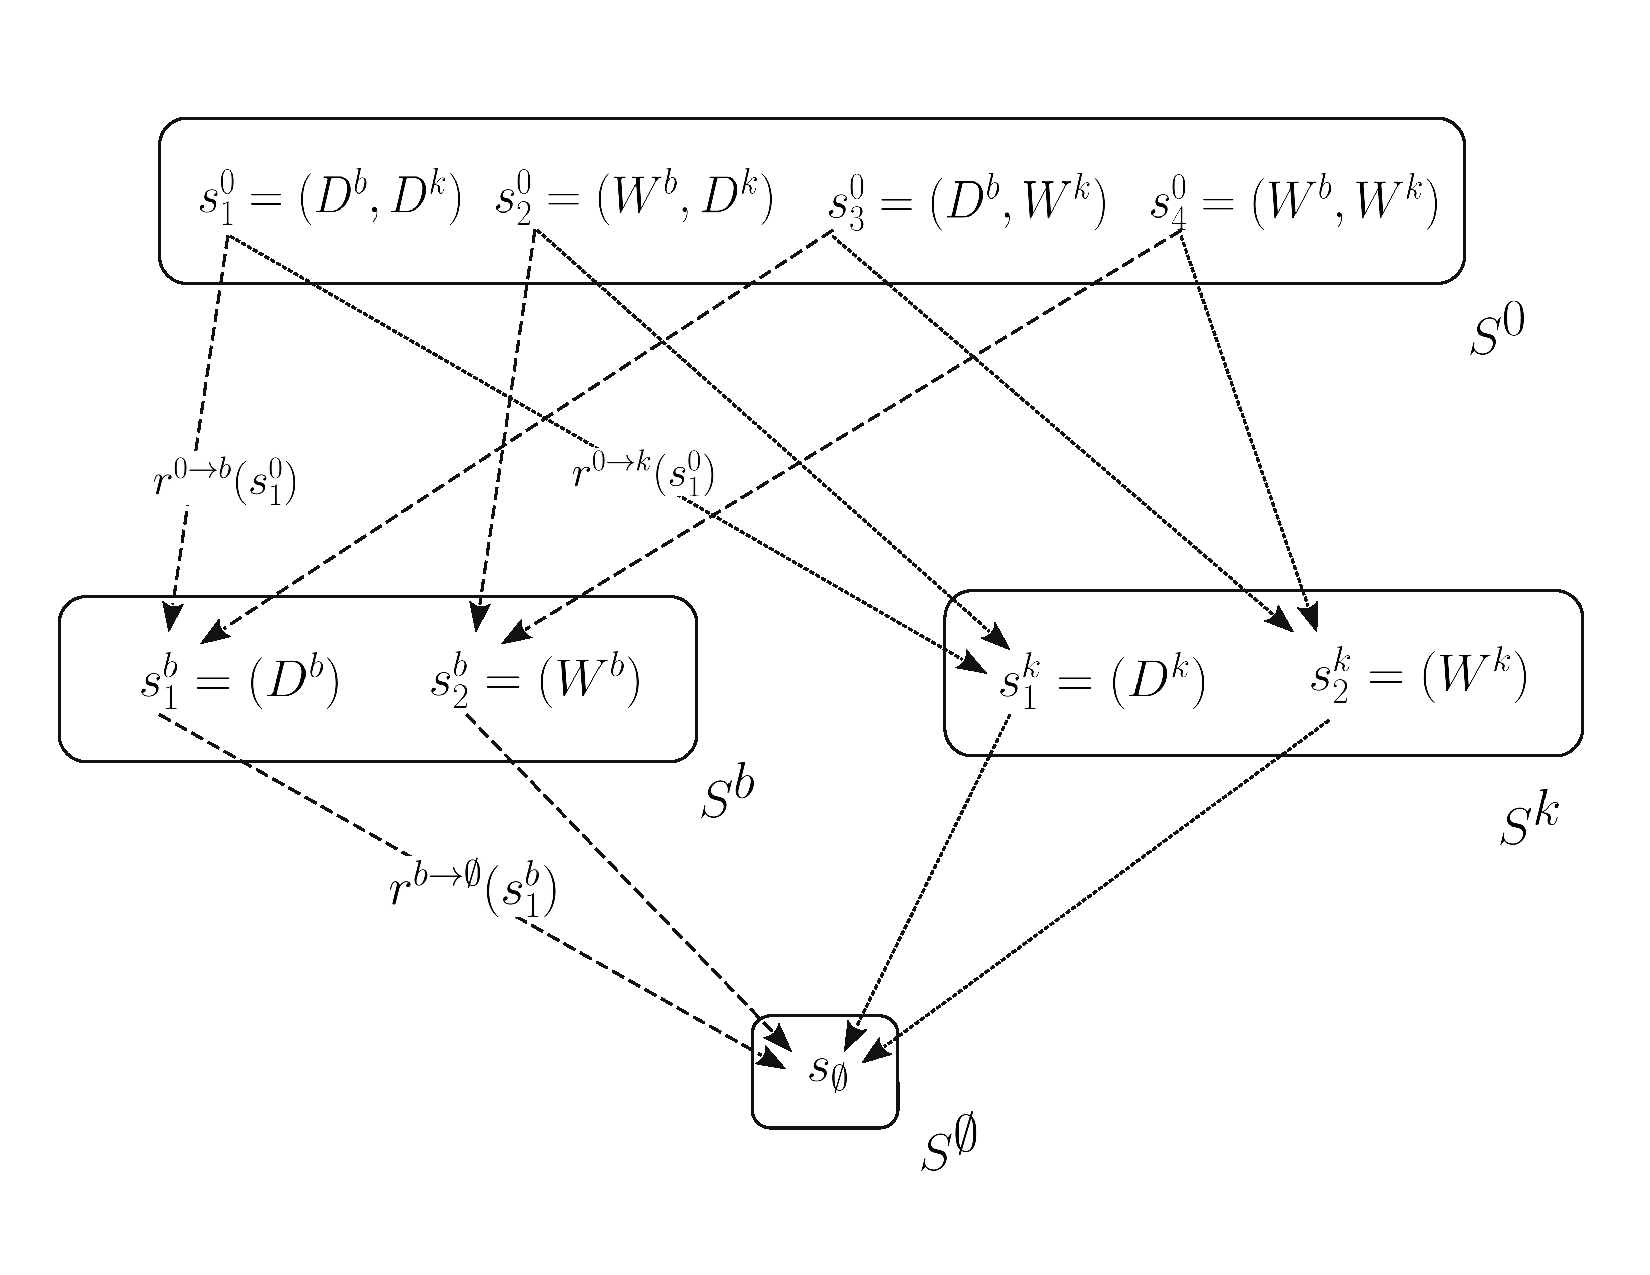
\includegraphics[scale=.4]{lattice.png}
	\end{center}
\caption{Awareness of Bob and Kate\label{fig:lattice}}
\end{figure}

To see a simple example of the setup, consider a situation in which  Bob ($b$) and Kate ($k$) live in different cities and are looking at their front lawns. 
The lawns are either dry ($D$) or wet ($W$).
Let $D^b$ and $W^b$ indicate that Bob's lawn is either dry or wet, respectively, and similarly for Kate. 
Then, in this simple world, Nature's state space is $S^0=\{s^0_1,s^0_2,s^0_3,s^0_4\}$, which are defined as shown in Figure \ref{fig:lattice}
Suppose Bob and Kate are aware of the status of their own lawns but not of each other's.
Then, Bob's state space is $S^b$, and Kate's is $S^k$.
The projections from $S^0$ to $S^b$ and $S^k$ are shown as are the ones from the latter two space to $S^\emptyset$.
(Not shown are the projections from $S^0$ to $S^\emptyset$.)

\begin{figure}[h!]	
	\begin{center}
		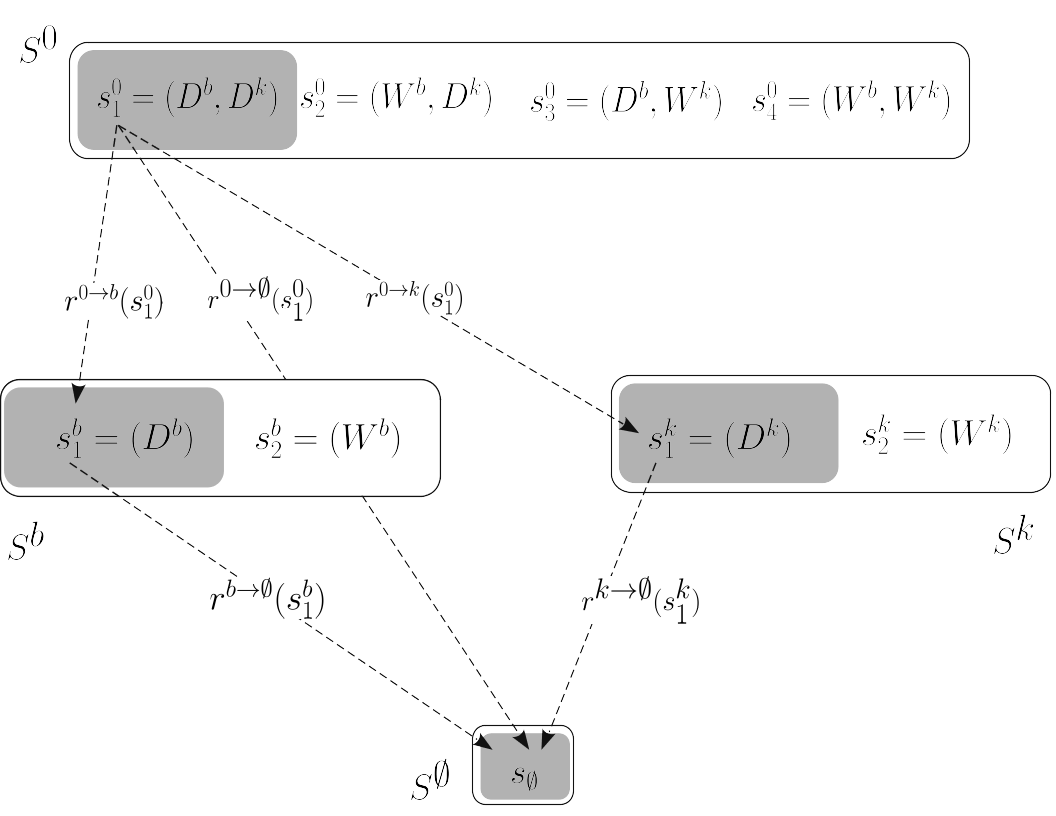
\includegraphics[scale=.4]{lattice-state.png}
	\end{center}
\caption{Awareness of state $S^0_1$ illustrated by the awareness diagram \label{fig:lattice-state}}
\end{figure}

Suppose state $s^0_1$ is actualized. 
Then, the projection functions map from this state to the awareness of each individual as well as to that of individuals of coarser awareness.
Fig. \ref{fig:lattice-state} illustrates the actualized state and all the projection sequences mapping from it.
For example,  $r^{0\rightarrow b}(s^0_1)$ maps $s^0_1$ in Nature's space maps to $s^b_1$ in Bob's space (as shown): when the state of the world is that both lawns are wet, Bob is only aware of the wetness of his own lawn.
In like fashion, $s^0_1$ maps to $s^k_1$ in Kate's space (as shown).
All states in Bob's and Kate's spaces map to $s^\emptyset$ in $S_\emptyset$.
Note that, while $S^0\succeq S^b\succeq S^\emptyset$ and $S^0\succeq S^k\succeq S^\emptyset$, $S^b$ and $S^k$ are neither richer nor poorer than the other -- they are not comparable.
We might imagine an individual living in a third city who is unaware of the states of both Bob and Kate's grass.
In this simple world, that individual would have complete unawareness -- i.e., would have a state space equal to $S^\emptyset$.
Keep in mind that the greyed areas in Fig. \ref{fig:lattice-state} showing what everyone is aware of is extracted from the information contained in Nature's actualized state, $s^0_1$.ig. \ref{fig:lattice-state}.
	
Alternatively, we can imagine a world in which Bob is the only individual.
Assume he can be in one of two places: Dallas ($D$) or Miami ($M$). 
He is aware of the wetness of the ground only in the geographic location in which he is present.
He is also aware of his location. 
The awareness structure consistent with this setup is illustrated in Figure \ref{Fig:Bob Location} (state and projection labels have been removed to reduce clutter).

\begin{figure}[h!]	
	\begin{center}
		\includegraphics[scale=.4]{Bob-Location.png}
	\end{center}
\caption{Bob's awareness is contingent on his location\label{Fig:Bob Location}}
\end{figure}

	
\subsubsection{Synchronic events}

The term `event' is used differently in philosophy than it is in probability theory. 
Since we are writing to audiences familiar with one or the other, it is important to clarify this difference. 
In probability theory, `event' is used similarly to the term `property' in philosophy, where properties are understood intensionally. 
Philosophers typically use `event' to mean a spatiotemporal particular extended over time. 
We refer to events associated with states at a moment in time (the game theory useage) as \textit{synchronic events}, and those associated with states unfolding through time (the philosophy usage) as \textit{diachronic events}.
Below, we define the former.
We wait to define the latter until Section \ref{sec:diachronic_setup}.
	
In probability theory, events are subsets of state spaces. 
For example, the event ``Mike intends to get a cup of coffee includes \textit{all} states in which getting a cup of coffee is the intention of Mike. 
In philosophical terminology, this is equivalent to the property \textit{being in a state in which Mike intends to get a cup of coffee,} where the intension of the property is all the states of the world in which the world exemplifies that property.
Because each individual is associated with a state space that elaborates states according to the features of the world of which that individual could be aware in a given moment, the events of which he or she could be aware are subsets of that space. 
For example, $B=\{s\in S^0|s\Rightarrow \text{Bob has a cup of coffee}\}$ is the event that collects all the states in Nature's space in which Bob has a cup of coffee.

Because individual state spaces may be related to one another and, in any case, are all related to reality fully elaborated ($S^0$), it will be helpful to associate events in $S^0$ with the awareness of the individuals of them.
For an event $B\subseteq S^0$, let $B^{\downarrow}=\bigcup_{S^j\in \mathcal{S}}\left(r^{0\rightarrow j}\right)^{-1}(B)$ be the extension of $B$ to include all states in the  individuals' state spaces consistent with the projection of $B$ into them.
Then, $E\subseteq \Sigma$ is a \textit{synchronic event} if it is of the form $B^{\downarrow}$ for some $B\subseteq S^0$.
We refer to the state space event, $B$, as the \textit{basis} of the sychronic event $E=B^{\downarrow}$.
	
By this definition, not every subset of $\Sigma$ is a synchronic event.
If $B\subseteq S^0$, define the negation of the synchronic event $B^{\downarrow}$, denoted $\lnot B^{\downarrow}$, as $(S^0\setminus B)^{\downarrow}$,  a  subset of $\Sigma\setminus B^{\downarrow}$.
Typically, $B\cap \lnot B$ is a strict subset of $\Sigma$; unlike the standard probability space setup, $2^\Sigma$ is not the event space.
Nevertheless, by our definition, $\lnot\lnot B^\downarrow = B^\downarrow$.\footnote
{
	This is not true in \citet{Heifetz2006}.
		The difference is our extended events are generated by events in a specific space (in their terminology, Nature's space is always the ``base space''), which is an added restriction that assures this nice technical feature.
}

\begin{figure}[h!]	
	\begin{center}
		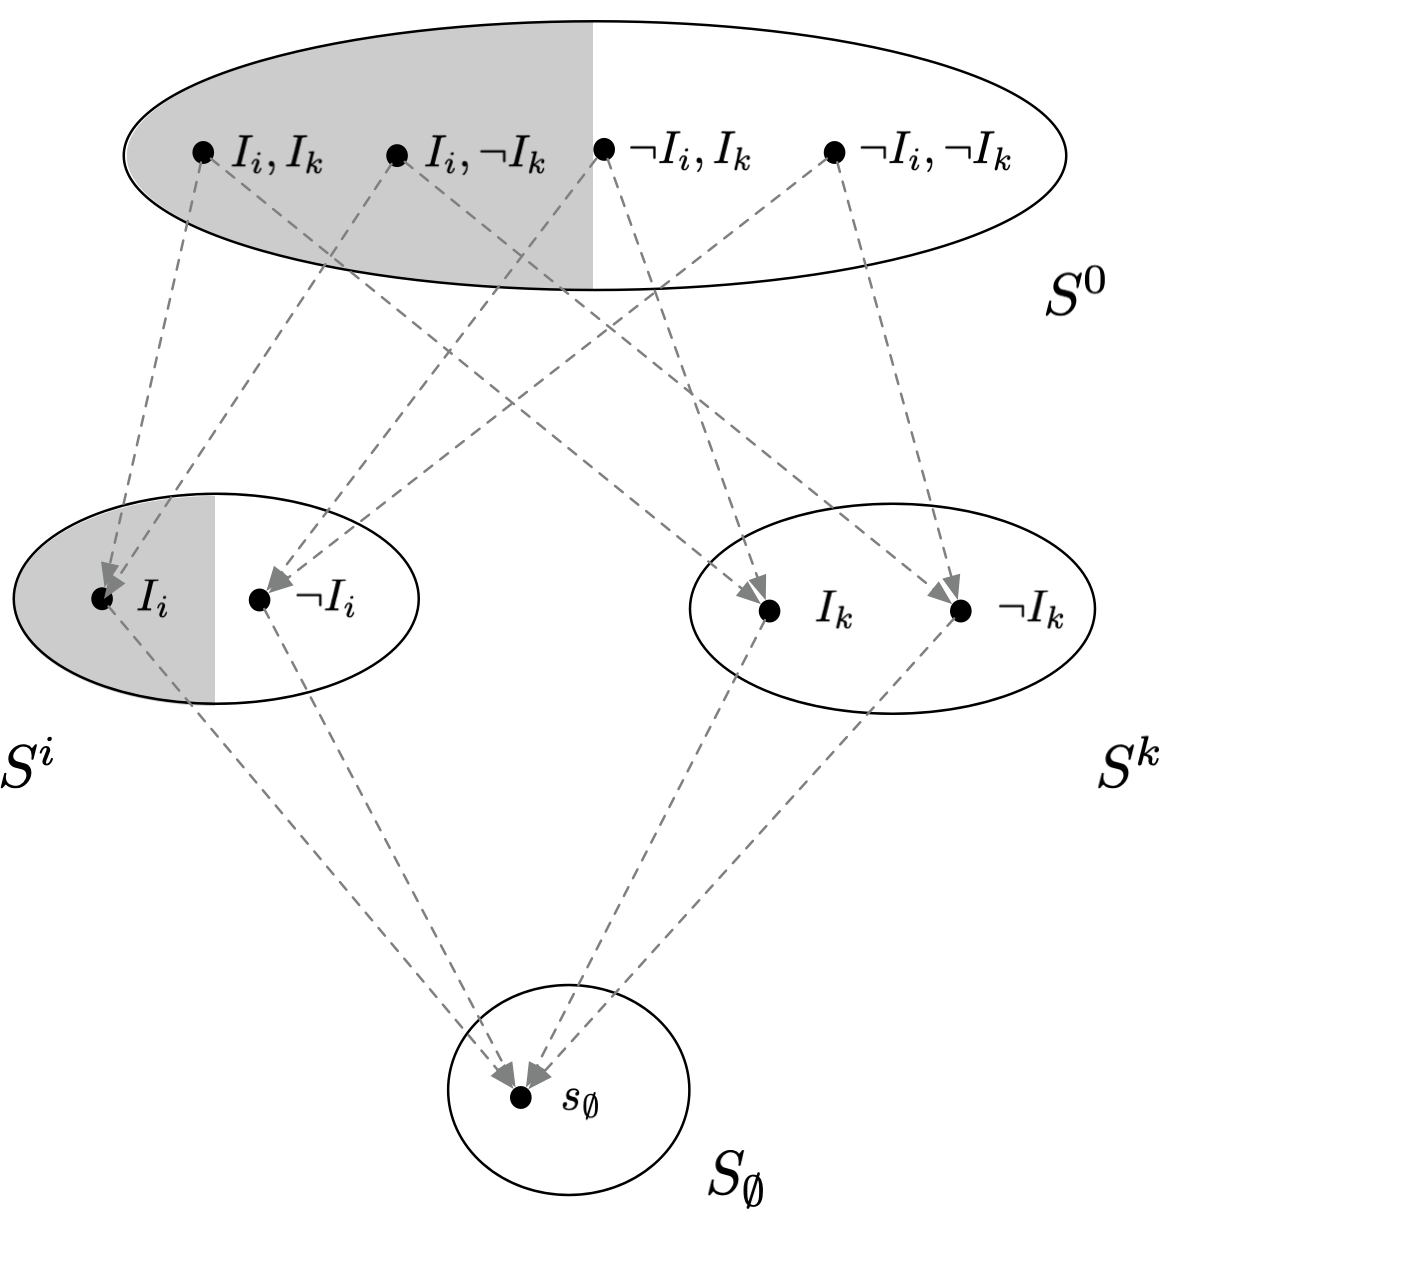
\includegraphics[scale=.4]{lattice-event.png}
	\end{center}
	\caption{The sycnronic event ``Kate's grass is wet'' with corresponding projections shown.\label{lattice-event}}
\end{figure}
	
Returning to our example with Bob and Kate, consider the event ``Kate's grass is wet' in $S^0$: $B=\{s^0_3,s^0_4\}$.
$B$ is the basis of $B^{\downarrow}=\{s^0_3,s^0_4,s^b_1,s^b_2,s^k_2,s^\emptyset\}$.
Notice that $\lnot B^{\downarrow}=\{s^0_1,s^0_2,s^b_1,s^b_2,s^k_1,s^\emptyset\}$.
Thus, $B^{\downarrow}\cup \lnot B^{\downarrow}=\Sigma$.
Here, the impossible event ``Kate's grass is both wet and dry'' corresponds to $\emptyset^{S^k}$.
	 

\subsection{Diachronic Awareness}\label{sec:diachronic_setup}

We now extend this framework to the dynamic setting.
Assume time is discreet and limit attention to some finite number of periods, $T$. 
Time subscripts are added to indicate the period. For example, \textit{Nature's state space at time} $t$, is denoted $S^0_t\subset S^0$, where with an arbitrary element denoted $s^0_t\in S^0_t$
Then, $S^0$ contains all the states that could possibly be actualized at $t$ expressed in their richest level of detail.
We continue to use index subscripts to identify specific states when necessary; e.g., $s^0_{3,t}$ is the state indexed as number 3 in Nature's state space in priod $t.$


\subsubsection{Acts and actions\label{sec:dynamics}}
The sequence of states actualized over the period of analysis is effected by the acts of the individuals in the population in conjunction with acts of Nature (i.e., all the causes that, in conjunction with the acts of the individuals, determine the actualization of a particular state from an immediately preceding, previously actualized state).
For each individual $i\in N$ and each state $s\in S^0$,  $A^i(s)$ indicates the set of \textit{feasible acts available to individual $i$ in state $s$} with arbitrary element $a^i\in A^i(s)$.\footnote
{
	Notice that we use a capital letter to indicate that $A^i$ is a set-valued function: $A^i:S^0\rightarrow 2^A$.
	Also note that feasible acts for individual $i\ne 0$ are determined by reality (states in $S^0$), not by $i$'s awareness of reality (states in $S^i$).
	Because we consider the intentional formation of some mental attitudes as choices available to individuals, we use the term ``act'' to describe the choices available to someone in a broad way.
	We think of ``action'' as describing the narrower category of act associated with physical movement.
} 
	
We adopt the convention that $A^i(s)=\emptyset$ indicates that individual $i$ has no available acts in state $s$.
An \textit{act profile} is a list of acts, one for each individual, denoted  $\mathbf{a}\equiv(a^0,\ldots,a^n)$. 
Recall, Nature is ``Individual 0'' so that $a^0$ summarizes all the developments that, in conjunction with the individuals' acts, determine which state is actualized following $s$. 
The set of \textit{all act profiles at state $s$} is $\mathbf{A}(s)\equiv \times_{i=0}^n A^i(s)$; the set of \textit{all possible act profiles at time $t$} is  $\mathbf{A}_t\equiv \cup_{s\in S^0_t} \mathbf{A}(s)$; and the set of \textit{all possible act profiles} is $\mathbf{A}\equiv \cup_{s\in S^0} \mathbf{A}(s)$. 


\subsubsection{Dynamics  } 
  
As indicated above, the act profiles summarize all the conditions required to actualize one state from the previously actualized state. 
To formalize this, let $\omega:\mathbf{A}\times S^0\rightarrow S^0$ be the \textit{state-contingent actualization function}, where $\omega(\mathbf{a}_t,s^0_t)=s^0_{t+1}$indicates that if the act profile at state $s^0_t\in S^0_t$ is $\mathbf{a}_t\in \mathbf{A}(s^0_t)$, then the next state actualized is $s^0_{t+1}$.
Notice that the engine of change operates at the level of Nature's reality: individuals find themselves in some true state $s^0_t$; 
they implement their human acts alongside Nature's act (this act elaborates the things that occur beyond the acts of the individuals represented in the analysis), as summarized by $\mathbf{a}_t$;
after which, the next state $s^0_{t+1}=\omega(\mathbf{a}_t,s^0_t)$ is actualized. 
Assume that, for all $t$, $\omega$ is bijective from $\mathbf{A}_t\times S_t$ to $S^0_t$.
In other words, each feasible  act profile in a given state at time $t$ leads to a unique state in period $t+1$ and each state in period $t+1$ can be traced back to a single predecessor state in period $t$ by a unique act profile that links the two.
Thus, the inverse $\omega^{-1}$ exists, where $\omega^{-1}(s^0_{t+1})=(\mathbf{a}_t,s^0_t)$ indicates if $s^0_{t+1}$ is actualized, then the immediately preceding state was $s^0t$ and $\mathbf{a}_t$ was the enacted act profile.
Suppose, for example, that two distinct sequences of acts could lead to an identical footprint in the snow.
In that case, we consider there to be two states in which that identical footprint exists, each associated with one of the sequences of acts that lead to it. 
The world begins at state $s_0^0$.
To allow for uncertainty or partial knowledge with respect to various aspects of the world at the beginning of time, we assume Nature's acts entirely determine $s^0_{1}$. 
That is, $\mathbf{a}_0=(a^0_0,\emptyset,\ldots,\emptyset)$, where $a^0_0$ represents all the actualized historic factors that lead individuals to their  first decision state, $s0_1=\omega(\mathbf{a}_0,s^0_0)$.
Uncertainty with respect to the state of the world in $t=1$ (e.g., about the intentions or other individuals) is, thus, formalized as uncertainty about ``Nature's act'' $a^0_0\in A^0(s_0)$ prior to the first decision period.

We define the \textit{history at state $s^0_t$} as a profile of states that starts at $s^0_0$ and ends at $s^0_t$, denoted $\mathbf{h}(s^0_t)=(s^0_0\ldots,s^0_t)$.
A history $\mathbf{h}(s^0_t)$ is \textit{feasible} if there exists a sequence of action profiles $\mathbf{a}_0,\ldots,\mathbf{a}_{t-1}$ such that $s^0_1=\omega(\mathbf{a}_0,s^0_),\ldots, s^0_t=\omega(\mathbf{a}_{t-1},s^0_{t-1})$.
Feasible histories are the only ones that can be actualized according to objective reality.\footnote
{
	This distinction allows for situations in which individuals subjectively consider infeasible histories to be possible. 
	For example, individual $i$ may believe that act $a^i_t\in A^i(s^0_t)$ is consistent with the actualization of $s_{t+1}$ even though $a^i_t$ is not in the profile $\mathbf{a}_t$ that leads from $s_t$ to $s_{t+1}$.
	We do not examine these cases in this paper.
}
	
	
The set of all \textit{feasible histories at time $t$} is $\mathbf{H}_T$ and the set of all subsets of histories is $\mathcal{H}_T$.
An arbitrary \textit{history at time $t$} is denoted $\mathbf{h}_t\in \mathbf{H}_t$, where we start with the \textit{null history} $\mathbf{h}^0_0=(s^0_0)$ at the beginning of time (so, $\mathbf{H}^0_0=\{\mathbf{h}^0_0\}$ and  $S^0_0=\{s^0_0\}$).   
Because there is a single root node and $\omega$ is a bijection, the set of paths in $\mathbf{H}_T$ form a tree.
Thus, $S^0$ can be partitioned according to  subsets of states corresponding to time periods: $S^0=S^0_0\cup\cdots\cup S^0_T$ and $S^0_0\cap\cdots\cap S^0_T = \emptyset$.
Note also that each $S_t$ implies a partition of $\mathbf{H}_T$ according to the sets of paths intersecting the states in $S_t$.

% As we elaborate below, we assume that the status of one's mental attitudes at time $t$ is a feature of the actualized state $s_t$. 
	% First, we define \textit{beliefs} as subjective conjectures about the likelihood of past events, the present state, and future events. 
	% Second, \textit{desires} are the individual's attitudes toward histories, represented as a partial order relation on $\mathcal{H}_T$. 
	% In other words, individuals consider both the sequences of states they experience as well as the acts that induce them.
	% For example, even though a junior faculty member may have the same degree of desire for tenure at her present institution in all states of the world in which that happens, some paths to tenure may be more costly than others depending upon the acts required to get there (both her own and others, including those by Nature).
	% Making  the desire relation a partial order on $\mathcal{H}_T$ implies a partial order on $H_T$ but also allows individuals to compare events in $\mathcal{H}_T$ (e.g., the event of gaining tenure vs.\ not).
	% Third, \textit{intentions} represent an agent's commitment to undertake a plan of action designed to actualize an event in $\mathcal{H}_T$. 
	% As we will see, others' perceptions of one's intentions will play a social role in our framework.


% When $t$ is a future state, an ``awareness of awareness'' complication arises.
% That is, does $r^{0\rightarrow i}_t(s^0_t)$ represent the all the features of $s^0_t$ of which $i$  would be aware in an objective sense?
% Or, does it represent the all the features of the world that $i$, in the present period, subjectively imagines she  could be aware of in period $t$?
% For example, Sam may believe that in the next moment, she can become aware of the temperature outside by checking the internet. 
% Yet, suppose Nature is going to crash her internet service with certainty.
% Then, Sam's presumption of future awareness is not correct. 
% The answer, according to our logic, is that $i$'s awareness of her future potential for awareness is a mental attitude that is also embedded within the \textit{present} state.
% Thus, if need be, we can extend $r^{0\rightarrow i}_t$ so that, for any $T\ge w\ge t$, $s^i_w=r^{0\rightarrow i}_t(s^0_t,s^0_w)$ represents $i$'s awareness in state $s^0_t$ about the future state $s^0_w$.



	 +++++++++++++++++++++++++++++++++++STOPPED HERE++++++++++++++++++++++
	

\subsubsection{Diachronic events}
	
	A \textit{diachronic event} is a subset $D\in 2^{\mathbf{H}_T}$; i.e., a subset of paths in the tree associated with $\mathbf{H}_T$.\
	Note that diachronic events are subsets of whole paths from $s^0_0$ to subsets of states in $S^0_T$. 
	Therefore, they do not have time subscripts.
	Let $\mathcal{D}\equiv 2^{\mathbf{H}_T}$ be the set of all diachronic events.
	Given the preceding discussion, every synchronic event $\sigma_t\in\Sigma_t$ is associated with a unique event $E\in \mathcal{E}$. 

	
	To see how we use states and understand how these objects work, consider the canonical example of rolling a six-sided die. 
	We use functions on $S^0$ to ``extract'' information from the states. 
	Here, for example, we can let $d(s^0_t)$ indicate the outcome of a die roll in state $s^0_t$: for all $s^0_t\in S^0_t$, $d(s^0_t)\in\{1,2,3,4,5,6\}$; i.e., $d$ maps from each state in $S^0_t$ to a number between 1 and 6, indicating the side of the die that landed up in that state (where $s^0_t$ includes \textit{all} features of the world besides how the die landed).
	Now, the synchronic event ``the die roll is even'' is described by $\sigma_t\in\Sigma_t$ such that $\Sigma_t\equiv\{s^0_t\in S^0_t|d(s^0_t)=2,4\text{ or }6\}$. 
	Alternatively, suppose $T=2$.
	Then, the diachronic event, ``snake-eyes were rolled'' is described by $E\in\mathcal{E}$ such that $E\equiv\{(s^0_0,s^0_1,s^0_2)\in \mathbf{H}_T|d(s^0_1)=d(s^0_2)=1\}$.
	


	
\subsection{Mental attitudes\label{sec:attitudes}}

\paragraph{Beliefs \label{para: beliefs}}
	Beginning with beliefs, let $\Delta(H)$ denote the set of all probability distributions on the set of histories. 
	Then,  $\mu_i:S\rightarrow \Delta(H)$ is a function that maps from states to individual $i$'s beliefs on histories $H$. 
	We write  $\mu_i^s$ to indicate $i$'s subjective probability distribution on $H$ at state $s$.
	This distribution induces a distribution on history events, $\mathcal{H}\equiv 2^H$. 
	Note that each $\mu_i^s$ induces a probability distribution on $S$.
	For example, the probabilities of the elements of $Z$ (terminal nodes) are equal to the probabilities of the complete histories they terminate. 
	The probability of some arbitrary state $s_t$ is equal to the sum of the probabilities of the complete histories running through it, and so on.
	Since all of this is implied by $\mu_i$, we will slightly abuse notation and write, e.g.,  $\mu_i^s(Z)=\mu_i^s(H)$, even though $Z\in \mathcal{S}$ while $H\in \mathcal{H}$.
	
	It is important to note that the existence of more than one element in $S_0$ means that individuals may be uncertain about which tree is the objective one and, hence, the true history they have experienced. 
	If so, they will be uncertain about which state they are in. 
	In addition, there will be uncertainty about how the future unfolds. 
	At the moment, we have the objective world starting at $s_0^\ast$ and unfolding in accordance with $\omega$ and the sequence of everyone's act choices. 
	Since  acts are free choices by individuals, it is possible they are selected randomly (``now, I will decide what to do by flipping a coin'').
	This includes acts of Nature.
	All of individual $i$'s speculation with respect to the history, state and unfolding of events is summarized by $\mu_i$.


Like in the case of incomplete information, we proceed by introducing probability distributions on state-spaces. For any state space $S \in \mathcal{S}$, let $\Delta(S)$ be the set of probability distributions on $S$. Even though we consider probability distributions on each space $S \in \mathcal{S}$, we can talk about probability of events that, as we just have seen, are defined across spaces. To extend probabilities to events of our lattice structure, let $S_{\mu}$ denote the space on which $\mu$ is a probability measure. Whenever for some event $E \in \Sigma$ we have $S_{\mu} \succeq S(E)$ (i.e., the event $E$ can be expressed in space $S_{\mu}$) then we abuse notation slightly and write
\begin{equation*}
\mu \left( E \right) = \mu \left( E\cap S_{\mu}\right).
\end{equation*}
If $S(E) \npreceq S_{\mu}$ (i.e, the event $E$ is not expressible in the space $S_{\mu}$ because either $S_{\mu}$ is strictly poorer than $S(E)$ or $S_{\mu}$ and $S(E)$ are incomparable), then we leave $\mu(E)$ undefined.

To model an agent's awareness of events and beliefs over events and awareness and beliefs of other groups, we introduce type mappings. Given the preceding paragraph, we see how the belief of an agent at state $\omega \in S$ may be described by a probability distribution over states in a less expressive space $S'$ (i.e., $S \succeq S')$. This would represent an agent who is unaware of the events that can be expressed in $S$ but not in $S'$. These events are ``out of mind'' for him in the sense that he does not even form beliefs about them at $\omega$:  his beliefs are restricted to a space that cannot express these events.

More formally, for every agent $i \in N$ there is a \textit{type mapping} $t_{i}: \Omega \longrightarrow \bigcup_{S \in \mathcal{S}} \Delta(S)$. That is, the type mapping of agent $i \in N$ assigns to each state $\omega \in \Omega$ of the lattice a probability distribution over some space. Now a state does not only specify which events affecting value creation may obtain, and which beliefs agents hold over those events, but also which events agents are aware of. Recall that $S_{\mu}$ is the space on which $\mu$ is a probability distribution. Since $t_i(\omega)$ now refers to agent $i$'s probabilistic belief in state $\omega$, we can write $S_{t_i(\omega)}$ as the space on which $t_i(\omega)$ is a probability distribution. $S_{t_i(\omega)}$ represents the \emph{awareness level} of agent $i$ at state $\omega$. This terminology is intuitive because at $\omega$ agent $i$ forms beliefs about \textit{all} events in $S_{t_i(\omega)}$.

For a type mapping to make sense, certain properties must be satisfied. The most immediate one is \textit{Confinement:} if $\omega \in S'$ then $t_{i}(\omega )\in \triangle \left( S \right)$ for some $S \preceq S^{\prime}$. That is, the space over which agent $i$ has beliefs in $\omega$ is weakly less expressive than the space contains that $\omega$. Obviously,  a state in a less expressive space cannot describe beliefs over events that can only be expressed in a richer space.  We also impose Introspection, which played a role in our prior discussion of incomplete information: every agent at every state is certain of her beliefs at that state. In AppendixXX, we discuss additional properties that guarantee the consistent fit of beliefs and awareness across different state-spaces and rule out mistakes in information processing.
% \begin{figure}[h!]	
% 	\begin{center}
% 		\includegraphics[scale=.4]{lattice3.jpg}
% 	\end{center}
% \caption{Unawareness structure\label{lattice3}}
% \end{figure}

It might be helpful to illustrate type mappings with an example. FigureXX depicts the same lattice of spaces as in FiguresXX and XX. In addition, we depict the type mappings for three different groups. At any state in the upmost space $S_{pq}$, the blue agent is aware of $p$ but unaware of $q$. Moreover, she is certain whether or not $p$ depending on whether or not $p$ obtains. This is modeled by her type mapping that assigns probability 1 to state $p$ in every state where $p$ obtains and probability 1 to state $\neg p$ in every state where $\neg p$ obtains. (The blue circles represent the support of her probability distribution that must assign probability 1 to the unique state in the support.) An analogous interpretation applies to the red agent except that she is an expert in $q$. In contrast, the green agent is aware of both $p$ and $q$ but knows nothing with certainty, modeled by her probabilistic beliefs in the upmost space that assigns equal probability to each state in it.\footnote{The example is taken from \citet{Schipper2016} who shows how a generalist (i.e., the green agent) emerges as an entrepreneur and forms a firm made of specialists (i.e., the blue or red agents) in a knowledge-belief and awareness-based theory of the firm using strategic network formations games under incomplete information and unawareness.}

Unawareness structures allow us to model an agent's awareness and beliefs about another agent's awareness and beliefs, beliefs about that, and so on. This is because, as in the incomplete information case,  beliefs are over states and states also describe the awareness and beliefs of groups.  Return to FigureXX. At state $pq$ the green agent assigns probability $1$ that the blue group is aware of $p$ but unaware of $q$. Moreover, he assigns probability $1$ to the blue agent believing with probability 1 that the red group is unaware of $p$.\footnote{We  note, it has been shown that under appropriate assumptions on spaces $S \in \mathcal{S}$ and the type mapping, unawareness structures are rich enough to model any higher order beliefs of agents (see the working paper version of \citet{Heifetz2013}).}
	
\paragraph{Desires \label{para: desires}}
	For all $i\in N$, define the state-dependent \textit{desire relation} such that, for all $s\in S$,   $D_i^s\subset P\times P$ where, $(p^\prime,p^{\prime\prime})\in D_i^s$ means that  individual $i$ in state $s$ desires the path $p^{\prime\prime}$ at least as much as the path $p^\prime$. 
	Having described the mathematical structure of desires, we use the more intuitive notation $p^\prime\preceq_i^s p^{\prime\prime}$, which is defined to mean $(p^\prime,p^{\prime\prime})\in D_i^s$. 
	We use $\prec_i^s$ and $\approx_i^s$ to indicate strict preference and indifference, respectively. 
	
	Why make preferences over paths? Because we assume individuals care about how they get to an end as well as the end itself. 
	To take a canonical example, a homeowner may have a renovated kitchen in mind as the desired end. 
	However, even if the kitchen specs are provided in extensive detail (so the owner knows exactly what the end will be), there may be many contractors who can deliver it. 
	In this case, assuming there are several contractors from which to choose, each of which identify with a different path with states encoding costs  at each step of the way and the final quality of the work, the owner's choice will be based upon the path (costs) as well as the final state (quality). 
	Similarly, an individual sensitive to the time value of money will prefer shorter paths to longer ones, other things equal. 
	Or, individuals may value portions of the paths themselves.
	For example, even though a student drops out of school (thereby, not completing the degree), he or she may nevertheless value the portion of the education that was completed. 
	Our approach allows for special cases in which all these details are elaborated as primitives of the situation. For our discussion, we simply assume preferences are over paths.    %When $s$ is understood from the context, we simply write, e.g., $E^\prime\preceq_i E^{\prime\prime}$, dropping the superscript. 
	

	\paragraph{Intentions \label{para: intentions}}
	
	Finally, define the state-contingent \textit{intention} for individual $i$ as a function $\gamma_i:S\rightarrow \mathcal{S}$, where $\gamma_i(s)=E$ means that in state $s$ individual $i$ intends event $E$. 
	We assume that individuals have desires and beliefs in all states, but not necessarily intentions. 
	The idea here is that, e.g., in some states Mike intends the end ``Mike has a cup of coffee'' and in others, Mike has yet to form intentions.
	We adopt the convention that $\gamma_i(s)=\emptyset$ means that $s$ is a state in which individual $i$ has not formed an intention. 
	We highlight that states may be differentiated only by changes in mental attitudes. 
	For example, it may be that the only change from $s_t$ to $s_{t+1}$ is $\gamma_i^{s_t}=\emptyset$ to $\gamma_i^{s_{t+1}}=E$.
	This suggests that the interval between time periods may be very short (measured in milliseconds).
	
	This raises the question of how an individual moves from being in a state without an intention to one in which the intention is formed. 
	Here, we can require an act of commitment to cement the intention. 
	That is, if $s_t$ is a state in which $i$ does not have an intention, then the set of feasible acts, $A^{s_t}_i$, can include an \textit{act to form the intention} to ``get a cup of coffee,'' which would then take him to a state $s_{t+1}$ in which $\gamma_i^{s_{t+1}}=X$ where $X$ contains all the states consistent with $i$ having a cup of coffee.
	
	For all $i\in N$, individual $i$'s \textit{mental attitudes} are summarized by a triple denoted $\theta_i\equiv(\mu_i,D_i,\gamma_i)$.\footnote
	{
		In setting up mental features in this way, we are following a version of the familiar ``type-space'' approach used in game theory \citep[See][]{Harsanyi1967, Mertens1985a}. 
	} 
	A \textit{profile of mental features} for all the individuals is given by the profile $\theta\equiv(\theta_1,\ldots,\theta_n)$. 
	Given our conventions, we can write $\theta_i(s)$ and $\theta^s$ without ambiguity.
	%The set of all such profiles is $\Theta$.
	
	

	

	\subsection{Consistency conditions\label{sec:consistencies}}
	
	Having structured the objects of interest, we now explore various conditions required to impose the regularities between the various mental attitudes and between those attitudes and the external world that are appropriate to a rational human being. 
	
	\paragraph{Reality Alignment\label{para: reality alignment}} 
	Beginning with the latter, our setup allows individuals to believe (place positive probability on) things that are not objectively true. 
	However, it is difficult to square rationality with someone whose beliefs are completely divorced from reality. 
	Therefore, we assume beliefs align with reality at least to some extent.
	\begin{condition}[Grain of Truth]\label{cond:grain of truth}
		For all $i\in N$, $s_t\in S$, $\mu_i^s(h^\ast_t)>0$.
	\end{condition}
	\noindent That is, rational individuals do not rule out the true state of affairs. 
	This implies that, although an indivual's beliefs about an event may be wildly inaccurate, that belief is not completely irrational: i.e., for all $W\in \mathcal{H}$ such that $\mu_i^s(W)>0$, $h^\ast_t\in W$. 
	Going in the other direction, for all $h^\ast_t\in H^\ast$, there exists some $W\in \mathcal{H}$ such that $\mu_i^s(W)>0$.
	This condition is not without controversy as it does rule out situations in which an individual is surprised by being confronted with a state of affairs he or she had previously thought impossible.
	There are formal approaches to dealing with such situations.
	For now, however, we sidestep such issues.
	
	\paragraph{Learning\label{para: learning}}
	We can also think of consistencies implied by learning. 
	Even with the Grain of Truth Condition in place, our setup presently allows a person's beliefs through time to be completely inconsistent in all ways except $\mu_i^s(h^\ast_t)>0$. 
	For example, suppose $X,Y\in \mathcal{H}$ and $\mu_i^{s_t}(X)=1$ and $\mu_i^{s_{t+1}}(Y)=1$ ($X$ and $Y$ contain all the states $i$ believes are possible in periods $t$ and $t+1$, respectively). 
	Then, even if $X$ and $Y$ are quite large, there is nothing in the setup preventing $X\cap Y= h^\ast_{t+1}$; i.e., the \textit{only} consistency from period to period is belief in the possiblity of the objectively true history.
	Such situations seem inconsistent with any reasonable concept of learning. 
	The following condition is a notion of learning that admits a wide range of learning models.
	For example, Baysian updating is consistent with this (though, by no means requred).
	\begin{condition}[Weak Learning]\label{cond: weak learning}
		Let $X,Y\in \mathcal{H}$. For all $i\in N$, $s_t,s_x\in S, x>t$, if $\mu_i^{s_t}(X)=1$ and $\mu_i^{s_x}(Y)=1$, then $Y\subseteq X$.
	\end{condition}
	\noindent Notice that learning is, indeed, weak in the sense that one may never learn anything ($Y=X$ through time).
	However, we imagine that as individuals experience the world, their grasp of it becomes more refined. 
	Again, this condition is also not without controversy since it seems to rule out ``conversion'' experiences in which an individual shifts from one worldview to another, apparently inconsistent worldview.
	Whether or not such experiences are, in fact, inconsistent with Condition \ref{cond: weak learning} we leave for another discussion.
	
	\paragraph{Introspection\label{para: introspecton}} 
	It seems reasonable to assume that an individual knows his or her own mental features (but may be uncertain of those of others). 
	For example, being certain of one's own beliefs rules out some peculiar mistakes in information processing (e.g., \citet{Geanakoplos1989}, \citet{Samet1990}). 
	As described above, the probability distribution representing an individual’s beliefs in may vary by state.  
	Introspection entails that, at any given state, the agent's belief assigns probability 1 to the set of states in which he has the same belief as in that state. Formally, 
	\begin{condition}[Introspection]\label{cond: introspection}
		For each agent $i \in N$ and  state $ s \in S$, the agent's belief at $s$, $\mu_i^s$, assigns probability 1 to the set of states in which  $i$ has precisely these beliefs: 
		$\mu_i^s(\{s^\prime \in S \mid \mu_i^{s^\prime} = \mu_i^s\})=1$. 
	\end{condition}
	
	\paragraph{Ordering of desires \label{para: desire ordering}} 
	It is also typical to add some structure to desires, namely that they be a partially ordered. 
	Formally, for all $i\in N$, $\preceq_i$ is a partial order relation on the set of paths, $P$; i.e., the following conditions hold for all paths in $\Gamma$:
	\begin{enumerate}
		\item $\forall  p^\prime\in S, (p^\prime,p^\prime)\in D(p)$: the relation ip reflexive,
		\item $\forall  p^\prime,p^{\prime\prime}\in p,(p^\prime,p^{\prime\prime})\in D(p)\wedge (p^{\prime\prime},p^\prime)\in D(p)\Rightarrow p^\prime=p^{\prime\prime}$: the relation ip antipymmetric,
		\item $\forall  p^\prime, p^{\prime\prime}, p^{\prime\prime\prime}\in p, (p^\prime,p^{\prime\prime})\in D(p)\wedge (p^{\prime\prime},p^{\prime\prime\prime})\in D(p)\Rightarrow  (p^{\prime},p^{\prime\prime\prime})\in D(p)$: the relation is transitive.
	\end{enumerate} 
	These conditions simply assume that there is a certain degree of consistency in an individual's desires over states. 
	
	\paragraph{Intentions\label{para: intentons}} 
	An intention differs from both beliefs and desires in that this mental attitude implies the individual possessing it has made a commitment to take action toward a desired end. 
	The desired end is an event, such as ``Mike buys a cup of coffee,'' which may be actualized by a large number of states of the world; e.g., buying at McDonalds, or at Starbucks, or alone, or with friends, or while believing the dark roast is probably sold out. Thus, in state $s$, the object of individual $i$'s intention is an event in $\mathcal{S}$. 
	It is not enough for an individual to simply intend some outcome. 
	Rather, we assume that at the time an intention is formed, it is coupled with a concrete plan of action designed to achieve the desired end. 
	
	To formalize this, for each individual $i$, define an \textit{action plan} as a function $\sigma_i:S\rightarrow A$ where $\sigma_i(s)=a_i\in A_i(s)$ indicates that when individual $i$ arrives at state $s$ she selects an act $a_i$ from the set of acts $A_i(s)$ available at that state. 
	Since every state has a single history leading to it, action plans may be history-contingent.
	Notice that, as defined, the action plan indicates what act the individual will implement at every state. 
	Of course, we do not expect the individual to have thought through a contingency plan for every state in the state space. 
	Rather, we impose a means-ends consistency condition on $\sigma_i$ that joins the action plan to the intention.
	
	\begin{condition}[Weak Means-Ends Consistency]\label{cond:weak M-E}
		Suppose individual $i$'s intention is given by $\gamma_i(s)=X\in\mathcal{S}$. 
		Let $P^s_X\subset P$ denote all the paths in $\Gamma$ that begin at $s$ and terminate in $X$. 
		Then $\sigma_i$ is said to be \textit{weak means-ends consistent with $\gamma_i(s)$} if at no state $s^\prime$ along any path in $P^s_X$ does $\sigma_i^{s^\prime}$ force actualization of a state $s^{\prime\prime}$ that is not on any path in $P^s_X$. 
		By ``force'' we mean that $\sigma_i^{s^\prime}$ indicates an act that actualizes some state outside of $P^s_X$ regardless of the acts of all the other individuals and Nature. 
	\end{condition}
	
	\begin{condition}[Strong Means-Ends Consistency]\label{cond:strong M-E}
		Suppose individual $i$'s intention is given by $\gamma_i(s)=X\in\mathcal{S}$. 
		Let $P^s_X\subset P$ denote all the paths in $\Gamma$ that begin at $s$ and terminate in $X$. 
		Then $\sigma_i$ is said to be \textit{strong means-ends consistent with $\gamma_i(s)$} if at every state $s^\prime$ along any path in $P^s_X$,  $\sigma_i^{s^\prime}$ forces actualization of a state $s^{\prime\prime}$ that continues along a path in $P^s_X$. 
		By ``force'' we mean that $\sigma_i^{s^\prime}$ indicates an act that actualizes some state on a path in $P^s_X$ regardless of the acts of all the other individuals and Nature. 
	\end{condition}
	
	In other words, Condition \ref{cond:weak M-E} says that the individual's plan never has him unilaterally driving the world to a state from which the intended event cannot be reached. 
	When this condition is met, it may nevertheless be the case that the world is driven to such a state. 
	However, this will need to be the result of the acts of others and/or Nature and nothing to do with the acts of individual $i$. 
	The strong form, Condition \ref{cond:strong M-E}, says that individual $i$ has a plan of action by which he can gaurantee his intended even regardless of what anyone else does.
	There is another case which is this: no matter what $i$ does, the intended $X$ will happen. 
	In this case, I do not think we would properly call $X$ intention. 
	
	We also need some rationality conditions that tie the preferences over paths to the action plan. 
	This is subtle because paths are determined by the entire act profile (i.e., and not just the acts of $i$. 
	So, how do you tie in preferences. One possiblity is to use $i$'s may have beliefs about what the other agents are going to do (remember all of this would be encoded in the states) and, based upon this, choose an action plan that implements the most preferred path possible given the plans of the others. 
	This would then tie beliefs, desires, intentions and plans of action together. 
	
	
	[STOP HERE]
	

\bibliography{library}

\end{document}

pdflatex: --aux--directory=build
bibtex: build/% -include-directory=build